\documentclass{minimal}
\usepackage{graphicx,color}
\usepackage[utf8]{inputenc}
\usepackage[papersize={418.00bp,314.00bp},text={418.00bp,314.00bp}]{geometry}
\begin{document}
\centering
% Title: gl2ps_renderer figure
% Creator: GL2PS 1.4.2, (C) 1999-2020 C. Geuzaine
% For: Octave
% CreationDate: Mon Dec 12 15:30:48 2022
\setlength{\unitlength}{1pt}
\begin{picture}(0,0)
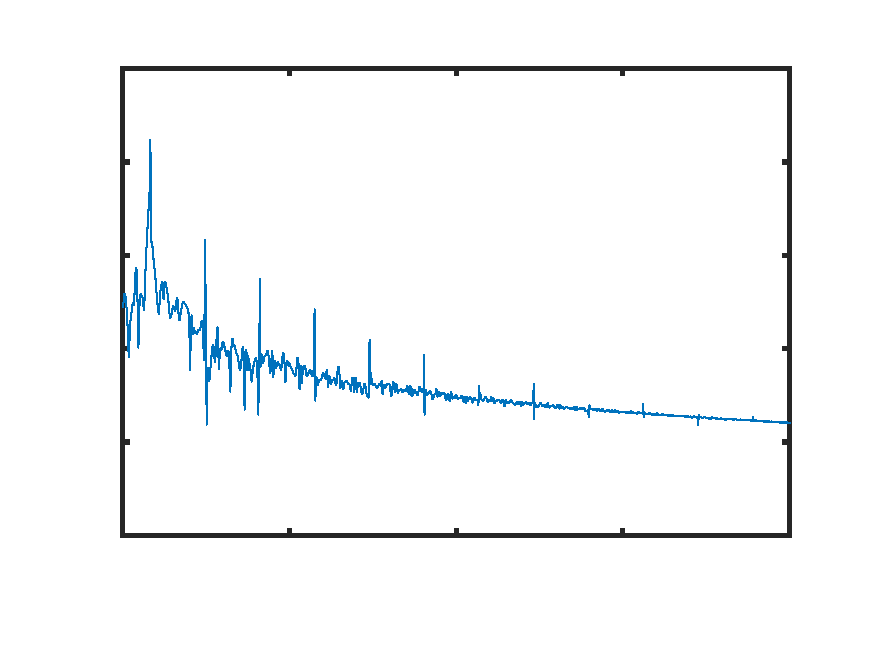
\includegraphics[scale=1]{DoubleFourierTheta1-inc}
\end{picture}%
\begin{picture}(418,314)(0,0)
\fontsize{20}{0}\selectfont\put(58.9984,41.956){\makebox(0,0)[t]{\textcolor[rgb]{0.15,0.15,0.15}{{0}}}}
\fontsize{20}{0}\selectfont\put(138.985,41.956){\makebox(0,0)[t]{\textcolor[rgb]{0.15,0.15,0.15}{{0.005}}}}
\fontsize{20}{0}\selectfont\put(218.972,41.956){\makebox(0,0)[t]{\textcolor[rgb]{0.15,0.15,0.15}{{0.01}}}}
\fontsize{20}{0}\selectfont\put(298.959,41.956){\makebox(0,0)[t]{\textcolor[rgb]{0.15,0.15,0.15}{{0.015}}}}
\fontsize{20}{0}\selectfont\put(378.946,41.956){\makebox(0,0)[t]{\textcolor[rgb]{0.15,0.15,0.15}{{0.02}}}}
\fontsize{20}{0}\selectfont\put(49,56.9588){\makebox(0,0)[r]{\textcolor[rgb]{0.15,0.15,0.15}{{0}}}}
\fontsize{20}{0}\selectfont\put(49,101.767){\makebox(0,0)[r]{\textcolor[rgb]{0.15,0.15,0.15}{{5}}}}
\fontsize{20}{0}\selectfont\put(49,146.575){\makebox(0,0)[r]{\textcolor[rgb]{0.15,0.15,0.15}{{10}}}}
\fontsize{20}{0}\selectfont\put(49,191.383){\makebox(0,0)[r]{\textcolor[rgb]{0.15,0.15,0.15}{{15}}}}
\fontsize{20}{0}\selectfont\put(49,236.192){\makebox(0,0)[r]{\textcolor[rgb]{0.15,0.15,0.15}{{20}}}}
\fontsize{20}{0}\selectfont\put(49,281){\makebox(0,0)[r]{\textcolor[rgb]{0.15,0.15,0.15}{{25}}}}
\fontsize{22}{0}\selectfont\put(218.972,21.956){\makebox(0,0)[t]{\textcolor[rgb]{0.15,0.15,0.15}{{Frequency}}}}
\fontsize{22}{0}\selectfont\put(22,168.979){\rotatebox{90}{\makebox(0,0)[b]{\textcolor[rgb]{0.15,0.15,0.15}{{log(Power Spectra)}}}}}
\fontsize{22}{0}\selectfont\put(218.972,291){\makebox(0,0)[b]{\textcolor[rgb]{0,0,0}{{Power Spectra of $\theta_1$}}}}
\end{picture}
\end{document}
